\chapter{Introduction}
\section{Energy storage}
\begin{itemize}
	\item Global warming
	\item EV
	\item Portable electronics
	\item Grid storage
\end{itemize}
\section{Lithium-ion batteries}
\begin{itemize}
	\item Why Li?
	\item Goodenough Schematic
	\item Explain the mechanisms underpinning batteries
\end{itemize}

\begin{figure}
\centering
\begin{subfigure}{\linewidth}
  \centering
  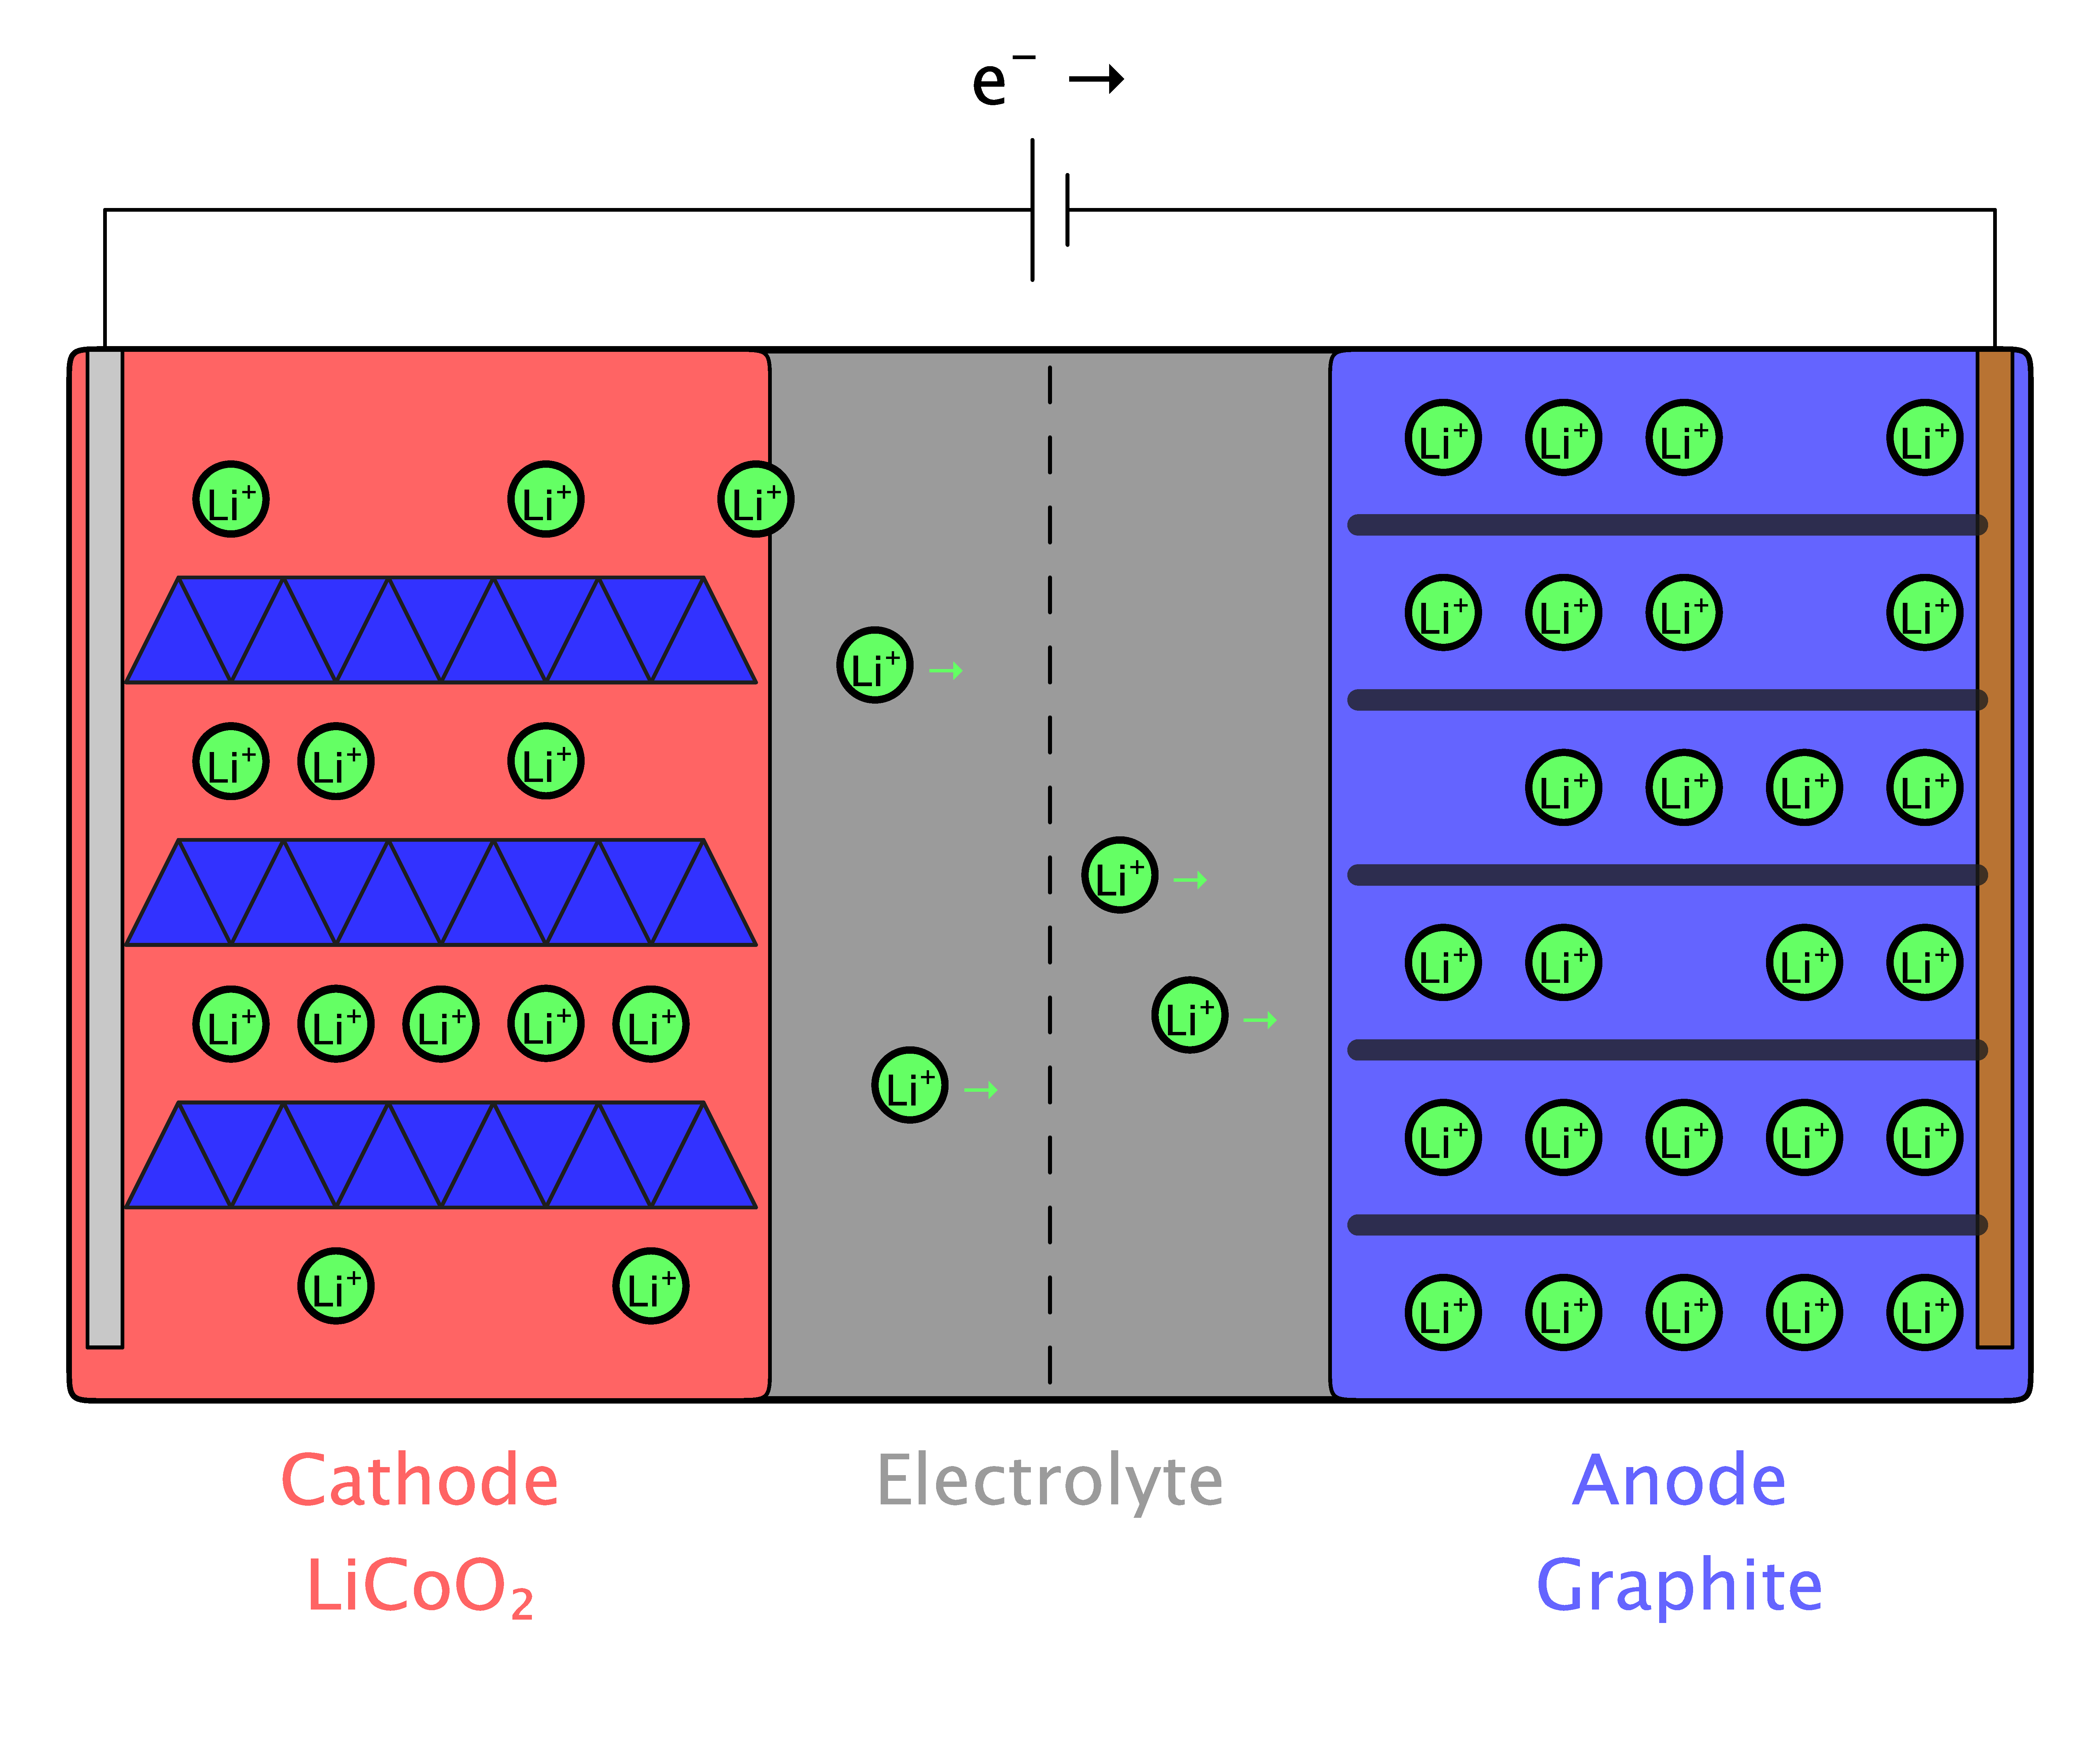
\includegraphics[width=0.7\linewidth, trim=1cm 1cm 1cm 1cm, clip]{figures/batteryCharge/batteryCharge}
  \caption{Charging}
  \label{fig:GoodenoughCharging}
\end{subfigure}

\begin{subfigure}{\linewidth}
  \centering
  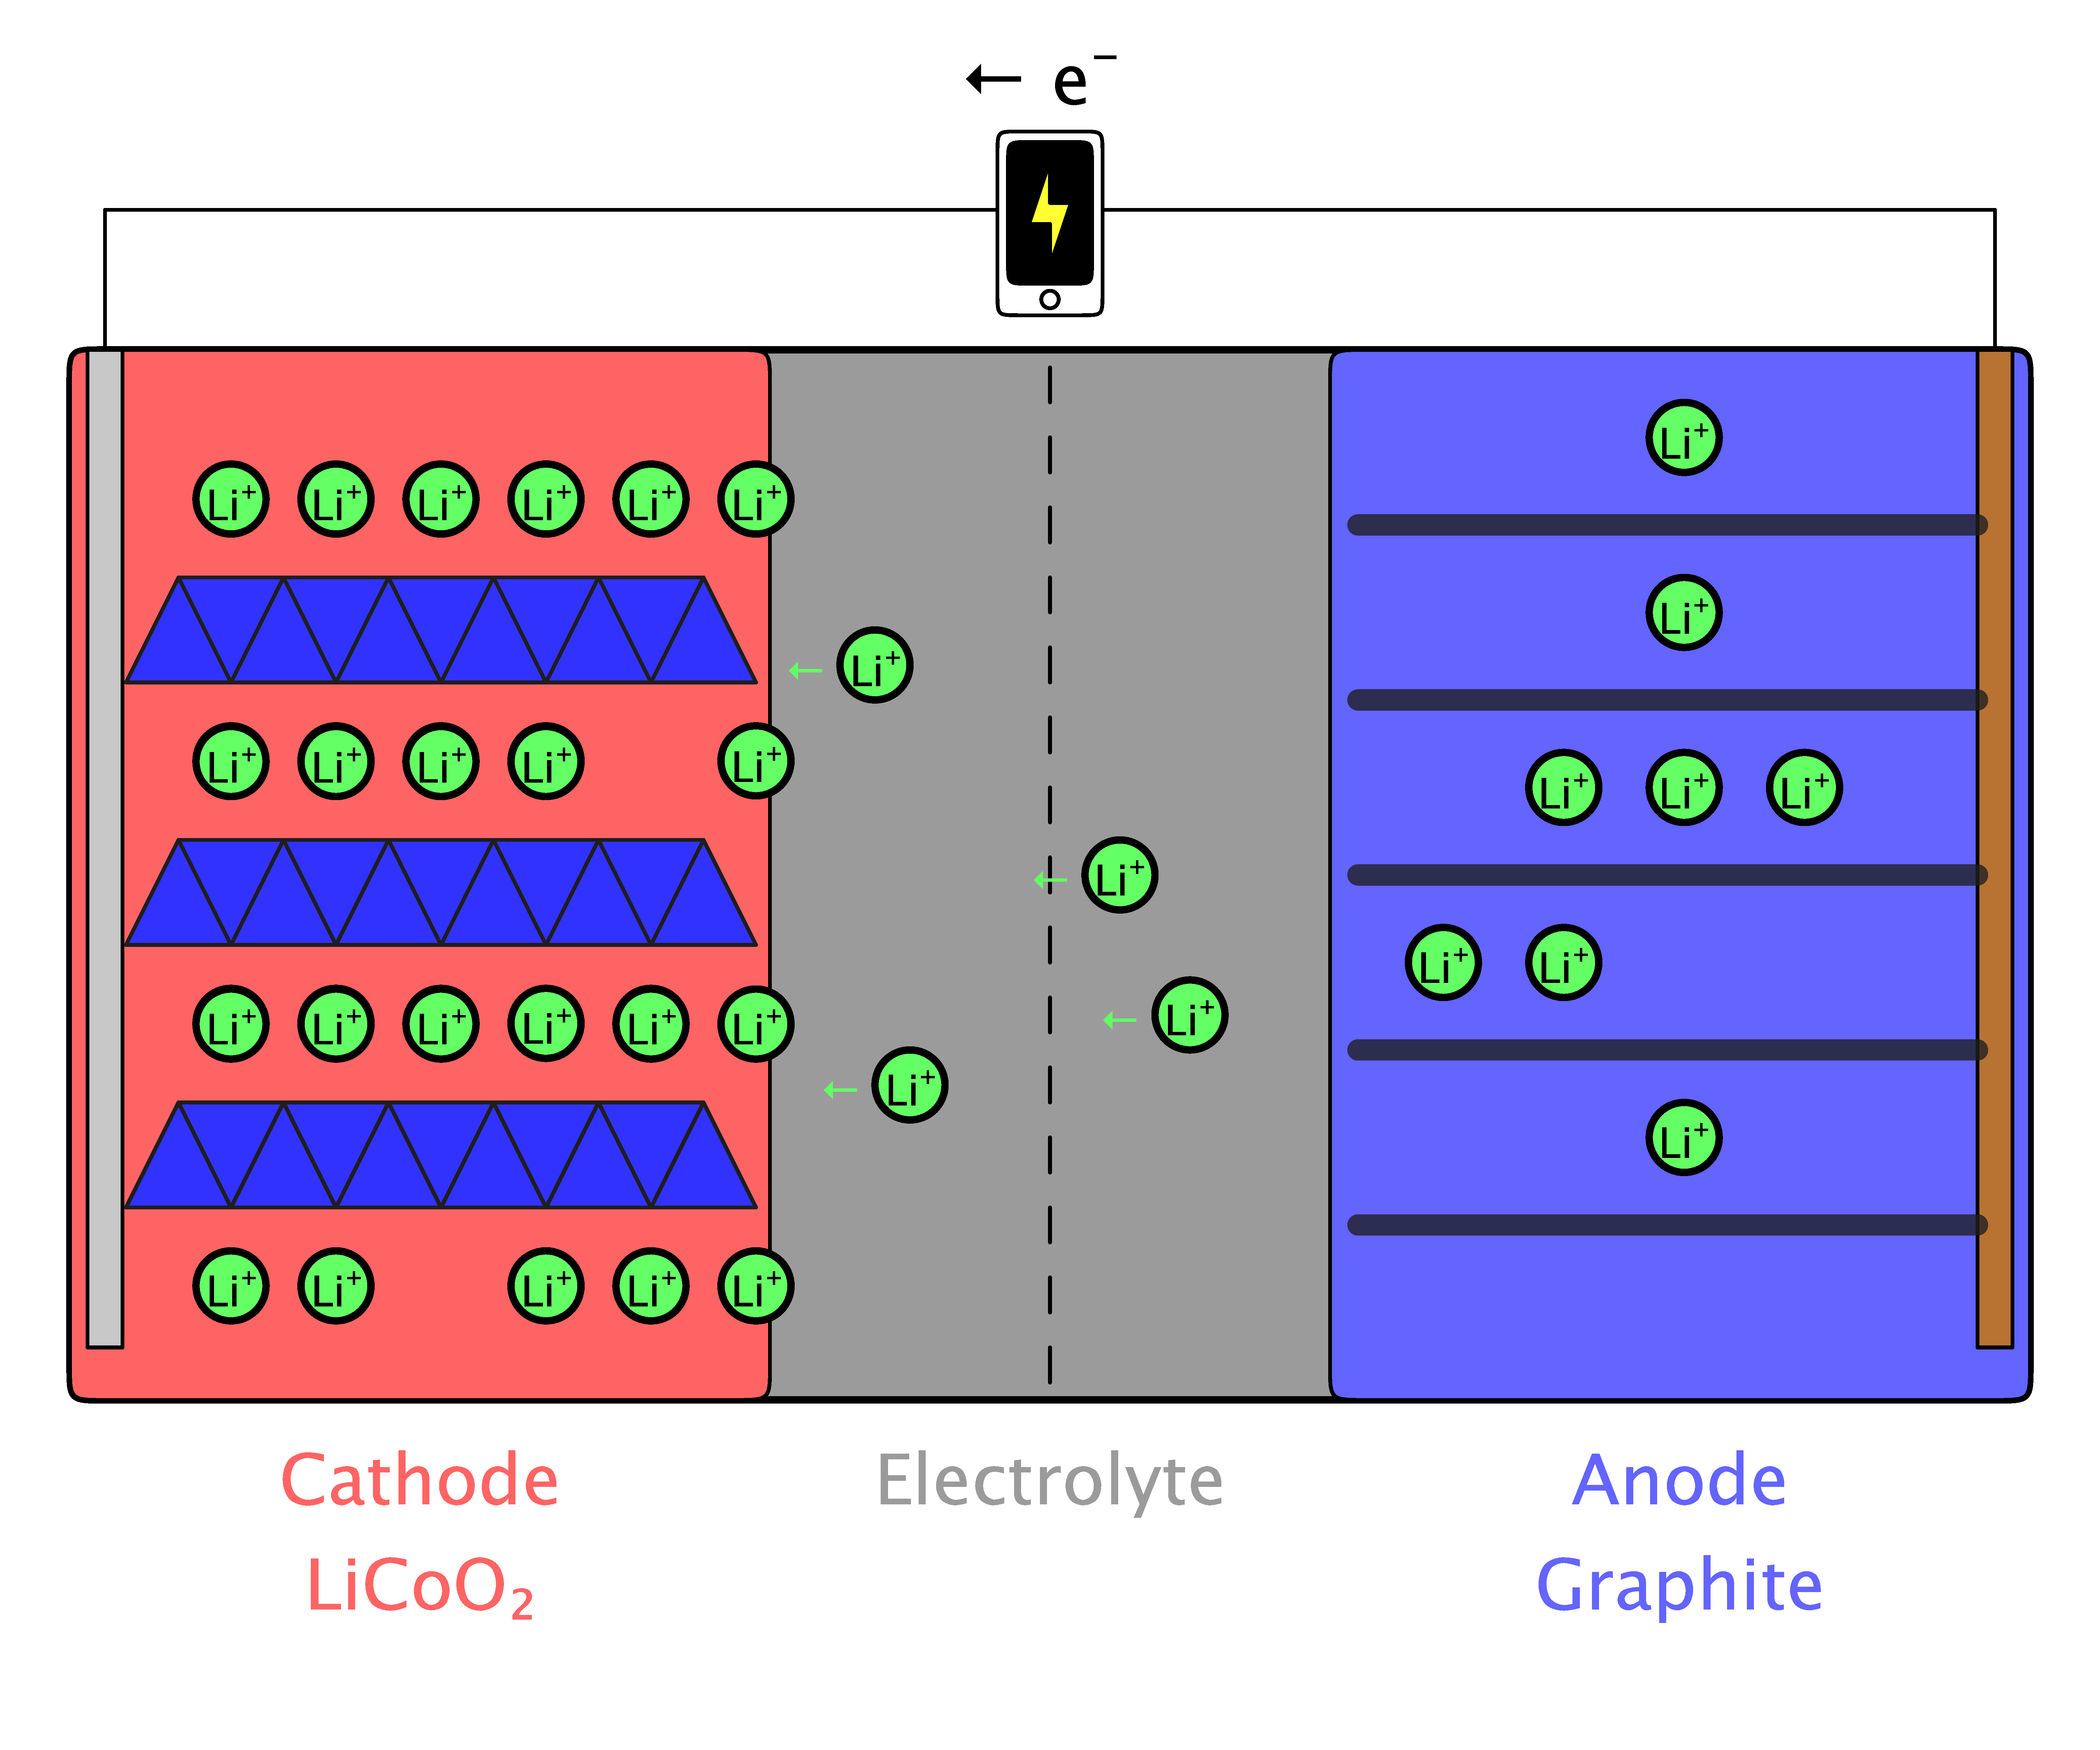
\includegraphics[width=0.7\linewidth, trim=1cm 1cm 1cm 1cm, clip]{figures/batteryDischarge/batteryDischarge}
  \caption{Discharging}
  \label{fig:GoodenoughDischarging}
\end{subfigure}
\caption[Li-ion battery schematic]{A schematic of a common Li-ion battery. During charging (a), electrons are driven to the anode by an external potential. \ce{Li+} ions move from the cathode to the anode to charge balance. During discharge (b), \ce{Li+} ions are driven to the cathode by a difference in chemical potential. The electrodes are electrically isolated by the separator, and are forced to instead travel via an external circuit and provide work.} 
\label{fig:Goodenough}
\end{figure}

\subsection{Alternatives}

\section{Electrolyte materials}
Explaination of electrolytes.
\subsection{Liquid electrolytes}
Currently widely used.
Significant concerns pertaining to safety, particularly for EV's.
Narrow stable voltage windows may be a limiting factor for newer cathodes.
\subsection{Solid electrolytes}
\citet{Bachman2016,Manthiram2017a,Janek2016,Famprikis2019,Zhang2018}
\section{Anode materials}
Li theoretically ideal.

Graphite commonly used

Metal oxides

Silicon

\section{Cathode materials}
\subsection{LiMO2}
LiCoO2

LiNiO2

LiMnO2

NMC

\subsection{LiFePO4}

\subsection{Spinel}

\subsection{Alternatives}
Na/Mg-ion

Li-air

\subsection{Limitations}

\section{Li-rich cathodes}

Motivation, definition.

Anion redox. \cite{Yahia2019}


\subsection{Li2MnO3}

\subsection{Li-rich NMC}

\subsection{Li4Mn2O5}
\subsection{Li2MnO2F}




